%%
%% This is file `xprintlen.tex',
%% part of the package xprintlen.
%%
%% Copyright (C) 2014 by Liam Huang <liamhuang0205+xprintlen@gmail.com>
%% --------------------------------------------------------------------------
%% This work may be distributed and/or modified under the
%% conditions of the LaTeX Project Public License, either version 1.3
%% of this license or (at your option) any later version.
%% The latest version of this license is in
%%   http://www.latex-project.org/lppl.txt
%% and version 1.3 or later is part of all distributions of LaTeX
%% version 2005/12/01 or later.
%%
%!TEX option = -shell-escape
%!TEX builder = latexmk
\documentclass{article}
\title{\bfseries The \textsf{xprintlen} package\thanks{This manual corresponds to \textsf{xprintlen.sty} v1.0, dated 2014/12/25}{\hspace{6pt}}\thanks{This work is released under the LaTeX Project Public
License (\url{http://www.latex-project.org/lppl.txt}), v1.3c or later.}}
\author{Liam Huang\thanks{\url{http://liam0205.me/}, \href{mailto:liamhuang0205+xprintlen@gmail.com}{liamhuang0205+xprintlen@gmail.com}}}
\date{2014/12/25}
\usepackage{mathpazo}
\usepackage{minted}
\usepackage{graphicx}
\usepackage{hyperref}
\hypersetup{hidelinks}
\usepackage{geometry}
\geometry{letterpaper, top = 1in, bottom = 1in}

\begin{document}
\maketitle

\section{Requirements}

\textsf{xprintlen} requires the package \textsf{fp} to be available and reasonably up to date on your system.

\section{Installation}

Put the \textsf{.sty} file into the folder \texttt{TEXMF/tex/latex/xprintlen}, and put other files into another folder \texttt{TEXMF/doc/latex/xprintlen}. Run \texttt{texhash} to refresh the file name data base.

\section{Usage}

This package defines a command, \verb|\printlen|, to print lengths in a variety of units. It supports all the units that \TeX{} supports, and its calculation depends on the package \textsf{fp}.

\verb|\printlen| recieves three parameters, while the first two parameters are the optionals. The first (optional) parameter sets the length of significant digits, whose default value is $ 2 $, stored in the marco \verb|\defaultsignificant|. The second (optional) parameter sets the unit to be print, and the default value of it is \texttt{mm}, stored in the marco \verb|\defaultunit|. The third parameter of the command, also the only mandatory parameter, is the length that will be calculated.

You can redefine the two marcos to revise the default length of significant digits and/or the default unit.

\section{Example}

\noindent\begin{minipage}[b]{0.55\linewidth}
The following lines will produce:

\begin{minted}{latex}
\documentclass{article}
\usepackage{xprintlen}
\newlength{\testlen}
\setlength{\testlen}{3.1415926cm}
\begin{document}
\obeylines
\printlen{\testlen}
\printlen[5]{\testlen}
\printlen[5][pt]{\testlen}
\end{document}
\end{minted}
\end{minipage}%
\begin{minipage}[b]{0.45\linewidth}
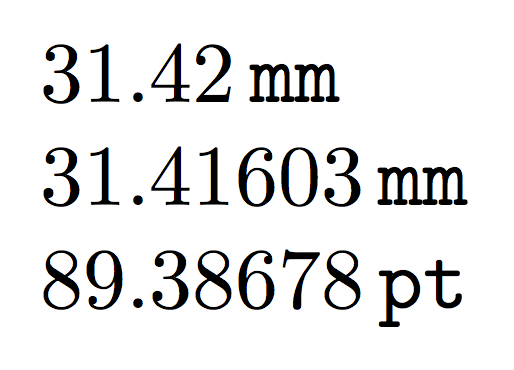
\includegraphics[scale = 0.6]{ex01}
\end{minipage}

\section{Change log}

\subsection*{Version 1.0, 2014/12/25}
\begin{itemize}
  \item The first public release.
\end{itemize}
\end{document}
